\section{Analyses of 6 networks}
\subsection{Available networks}
For this assignment, out of the 7 available networks, the ones I chose to work with are networks 1 through 5, and 7.

Before describing each network individually, one characteristic all of them share is that the edges in all 7 graphs are unweighted for the same reason. The questions asked \textit{"which people?"}, meaning that for each person in the list, you only place an edge if the answer is yes. Because it is binary (edge or no edge), all graphs have unweighted edges. However, if we had a question asking \textit{"how many times?"}, then there is a possibility of having weighted edges. Also, Gephi does not render a node if its degree equals zero.

\subsubsection{Network 1}
\begin{figure}
    \centering
    \subfloat[\centering Network 1]{{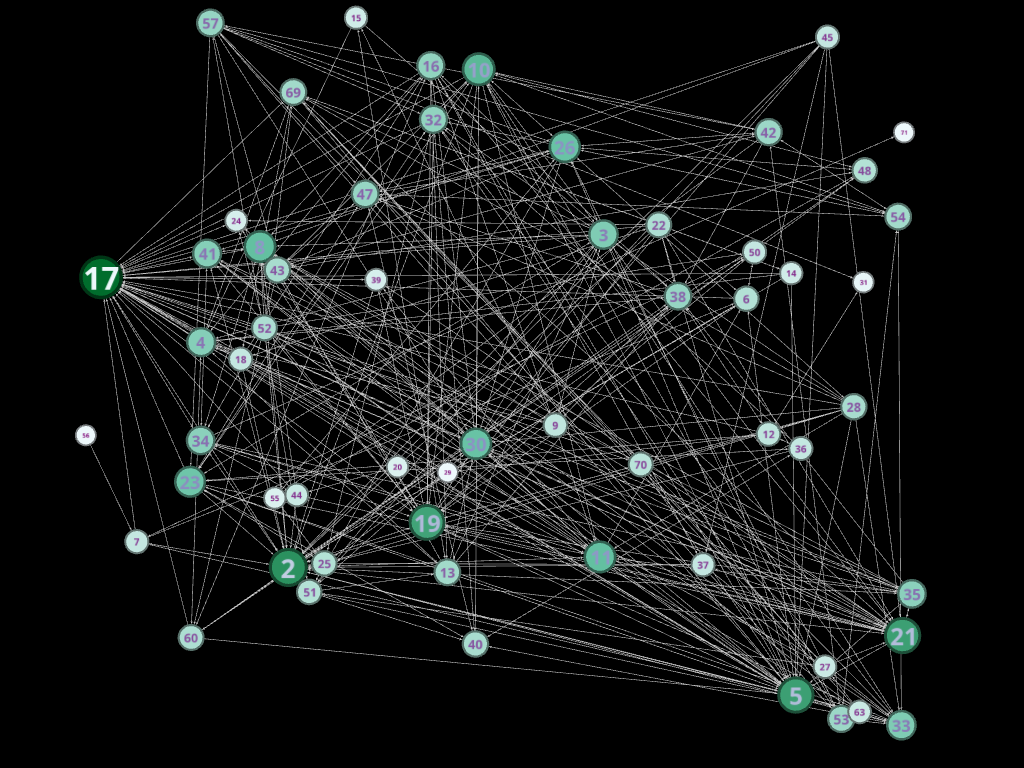
\includegraphics[width=0.45\textwidth]{img/net_0.png}}}
    \qquad
    \subfloat[\centering Network 2]{{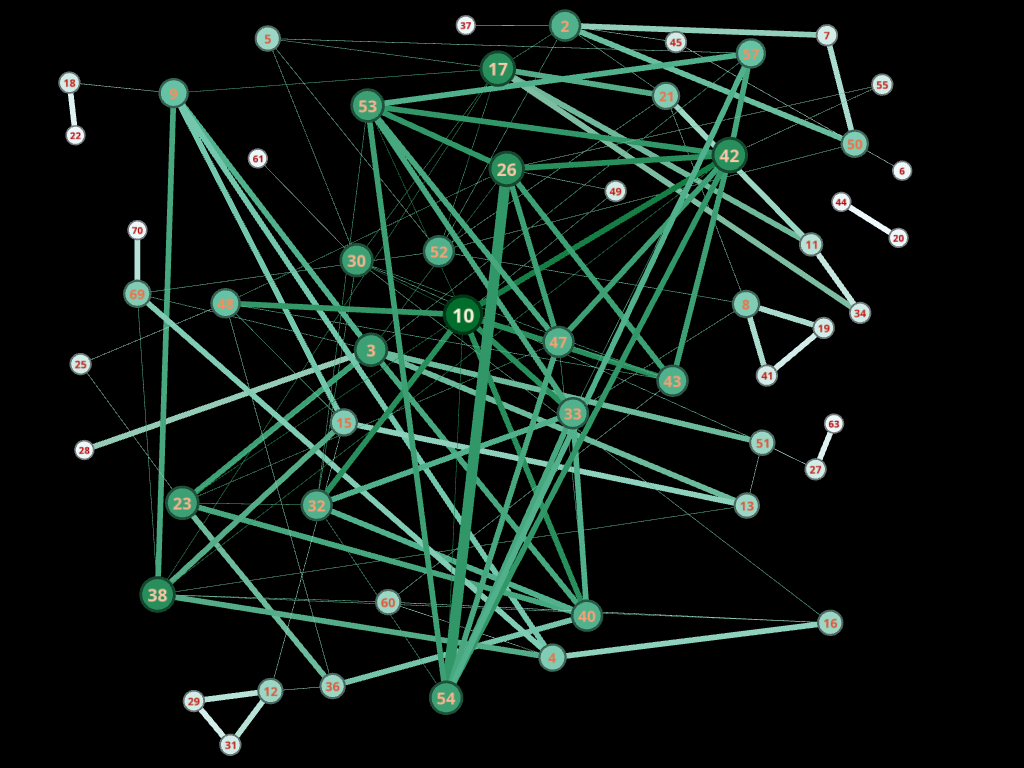
\includegraphics[width=0.45\textwidth]{img/net_1.png}}}
    \caption{Networks 1 \& 2}
    \label{fig:1}
\end{figure}

The first network asks the following question: \textit{"Which person you have hear of their voice or seen their faces?"}.

\textbf{Directed or undirected?} This network is an example of a directed graph. The reason for this is that in online conferences, it is not all participants who speak and/or have their computer cameras on. Therefore, I may see other people's faces and/or hear their voices, but they may not see or hear me.

\subsubsection{Network 2}
The second network asks the following question: \textit{"Which person you have met (in person+online) and exchange conversation?"}.

\textbf{Directed or undirected?} This network is an example of an undirected graph. In order to have a conversation, both parties must engage. If only one of them speak, there is no dialog. Therefore, is is not possible to exchange conversation.

\subsubsection{Network 3}
\begin{figure}
    \centering
    \subfloat[\centering Network 3]{{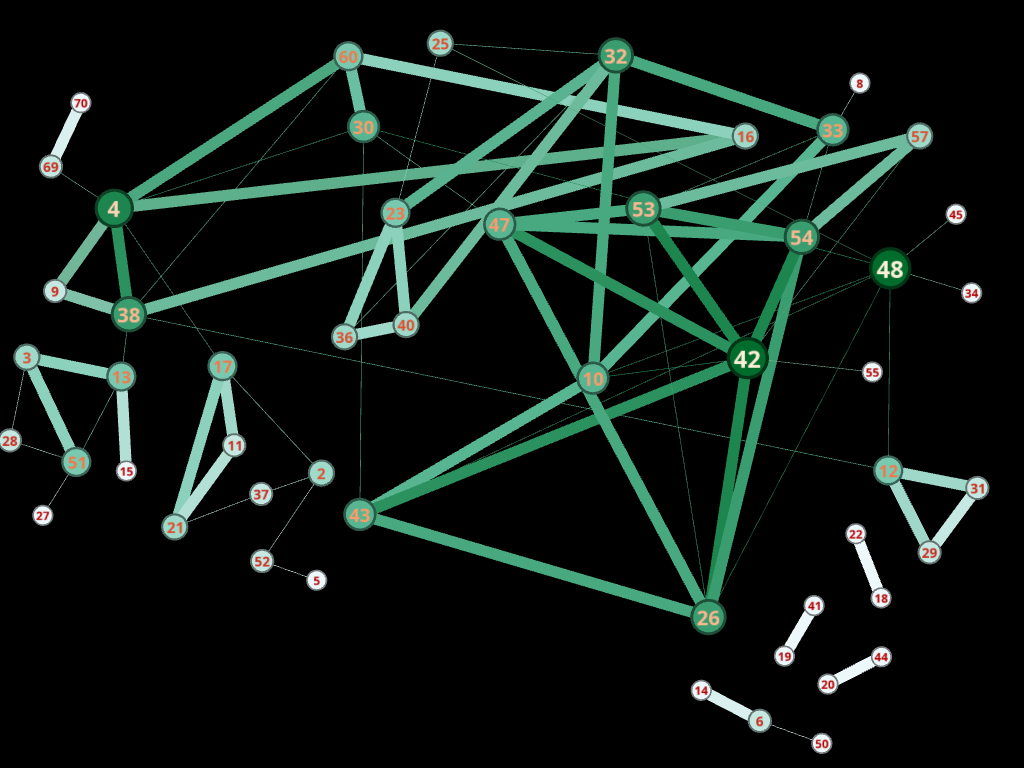
\includegraphics[width=0.45\textwidth]{img/net_2.png}}}
    \qquad
    \subfloat[\centering Network 4]{{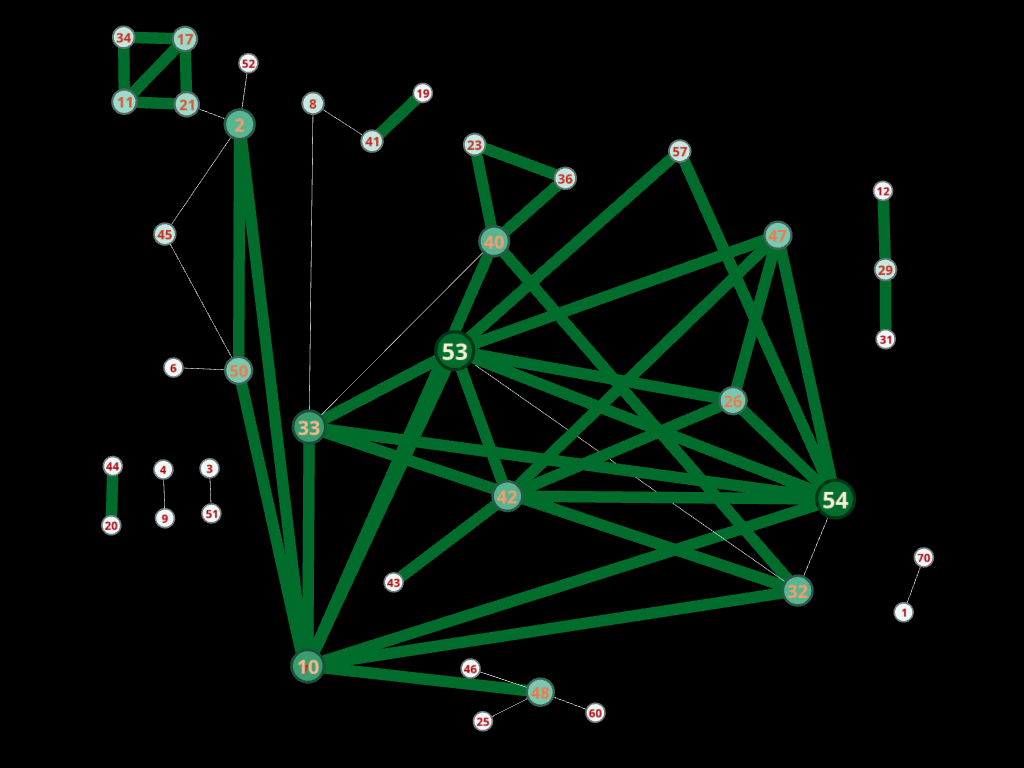
\includegraphics[width=0.45\textwidth]{img/net_3.png}}}
    \caption{Networks 3 \& 4}
    \label{fig:2}
\end{figure}

The third network asks the following question: \textit{"Which person you have collaborated with?"}.

\textbf{Directed or undirected?} This is an undirected graph because collaboration must be enforced by both parties. It has to be a mutual agreement.

\subsubsection{Network 4}
The fourth network asks the following question: \textit{"Which person you have eye contact?"}.

\textbf{Directed or undirected?} This network is undirected because in order to establish eye contact, two people must engage. There is no way for one person to look into someone else's eyes and not be looked back.

\subsubsection{Network 5}
\begin{figure}
    \centering
    \subfloat[\centering Network 5]{{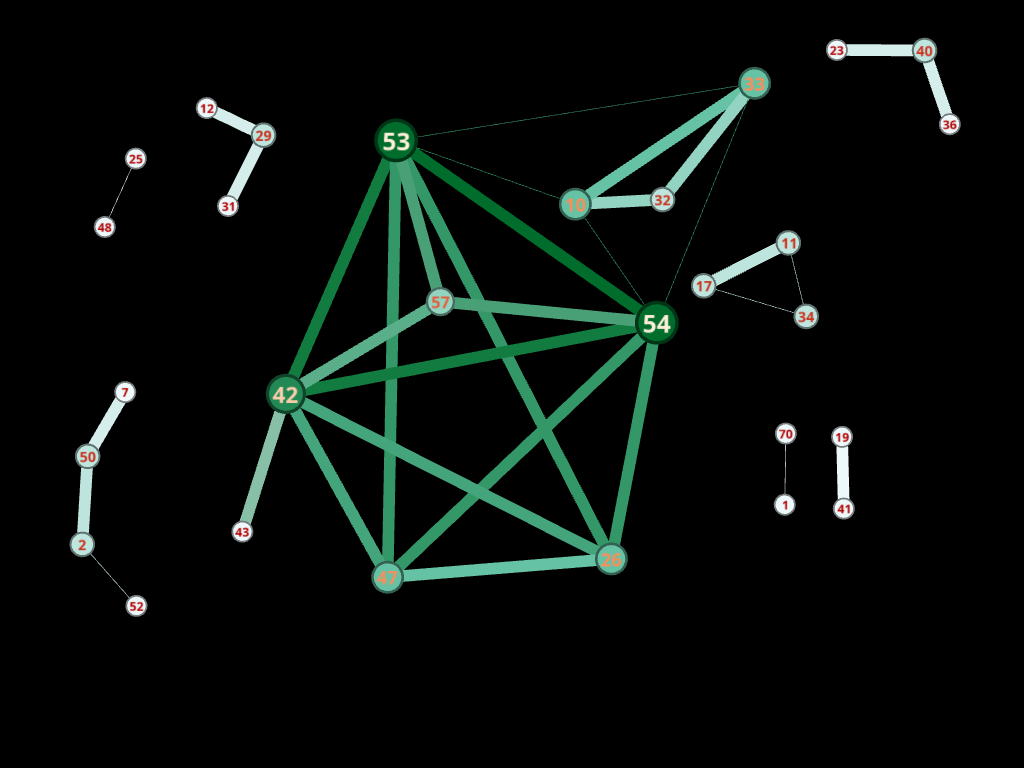
\includegraphics[width=0.45\textwidth]{img/net_4.png}}}
    \qquad
    \subfloat[\centering Network 7]{{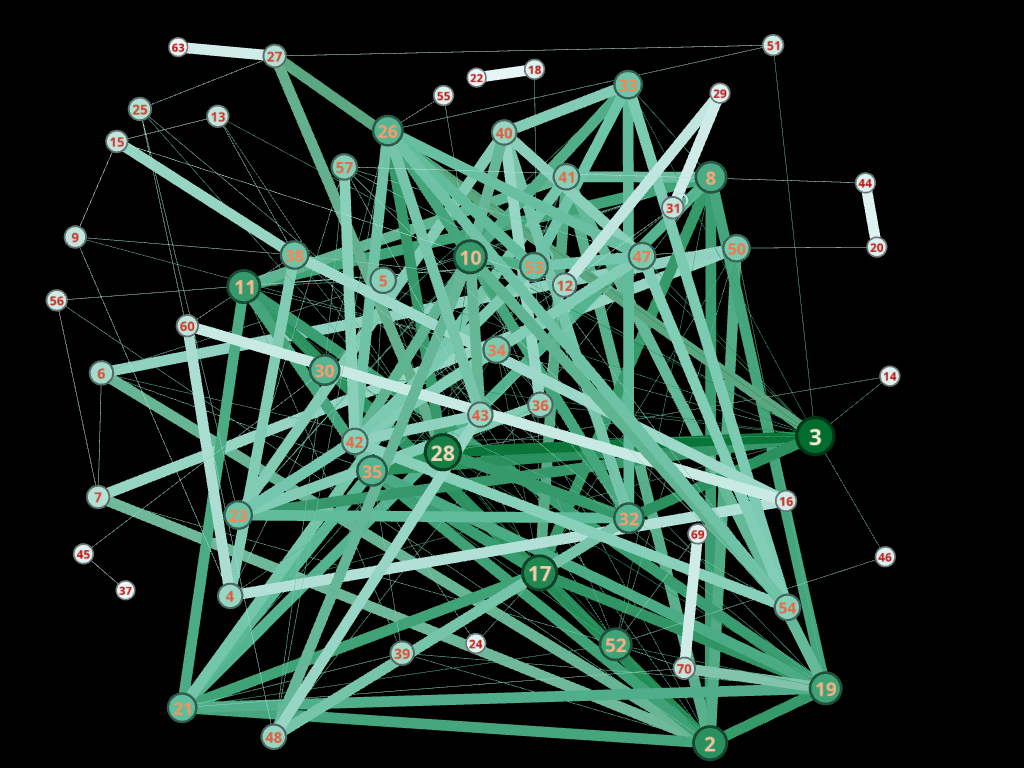
\includegraphics[width=0.45\textwidth]{img/net_6.png}}}
    \caption{Networks 5 \& 7}
    \label{fig:3}
\end{figure}

The fifth network asks the following question: \textit{"Which peson you have eaten lunch with?"}.

\textbf{Directed or undirected?} This is an undirected graph because eating lunch with another person implies that both people had to simultaneously engage in the activity.

\subsubsection{Network 7}
The seventh network asks the following question: \textit{"Which person you have taken at least two courses with?"}.

\textbf{Directed or undirected?} This network is an undirected graph because you cannot be simultaneously enrolled in a course another person has not and consider that as taking a course together. Also, the course must be taken in the same year.